\clearpage
\section{手推轮椅主体(Manual Propelled Wheelchair) 框图建模}

%%%%%%%%%%%%%%%%%
\begin{figure*}[h]
	\centering
	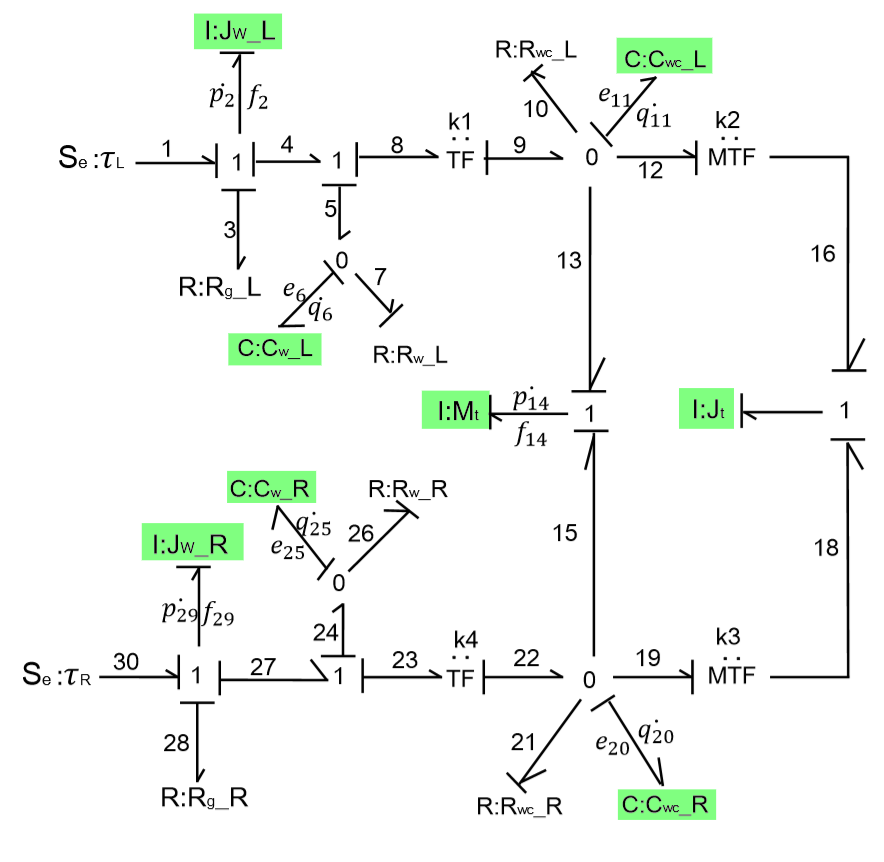
\includegraphics[width=0.7\textwidth]{fig/MPW.png}
	\caption{MPW因果化标注。}\label{fig:mdm}
\end{figure*}
%%%%%%%%%%%%%%%%%

\subsection{状态空间方程推导}

\begin{enumerate}

\item {后轮与地面运动状态变量$\dot{p}_2 $}

%%%%%%%%%%%%%%%%%
\begin{figure*}[h]
	\centering
	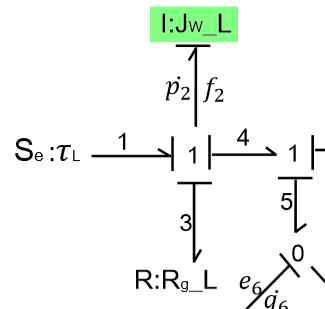
\includegraphics[width=0.4\textwidth]{fig/2_equation1.png}
\end{figure*}
%%%%%%%%%%%%%%%%%

对于$\dot{p} _ { 2 }$,开始列写方程,利用键合图的因果关系求出$e_2$:根据功率流方向标注,势变量$e_2$来自1结的输出,是由$e_1$,$e_3$,和$e_4$产生的,因此:

\begin{equation}\label{2_e2}
\dot{p}_{2}
=
e_2
=
e_1
-
e_3
-
e_4
=
\tau_L
-
e_3
-
e_4,
\end{equation}

$e_1$是输入变量,一直保留在最终的方程中;$e_3$来自阻性元件$R _ { eL }$的输出;$e_4$直接与状态变量有关,故而有下面三式:
\begin{equation}\label{2_e3}
e_3
=
f_3 \cdot R_{gL}
=
f_2 \cdot R_{gL}
=
\frac{p_{2}}{J_{wL}} R_{g L},
\end{equation}

\begin{equation}\label{2_e4}
e_4 = e_5 + e_8
=
e_6 + e_9 \cdot k_1
= 
\frac{q_{6}}{C_{wL}}
+
\frac{q_{11}}{C_{wcL}} k_{1},
\end{equation}

由式(\ref{2_e2})-(\ref{2_e4})得到状态方程1:
\begin{equation}\label{2_p2}
\dot{p}_{2}
=
\tau_{L}
-
\frac{p_{2}}{J_{wL}} R_{g L}
-
\frac{q_{11}}{C_{wcL}} k_{1}
-
\frac{q_{6}}{C_{wL}},
\end{equation}

%%%%%%%%%%%%%%%%%%%%%%%%%%%%%%%%%%%%%%%%%%%%%%%%%%%%%%%%%%%%%%%%
%%%%%%%%%%%%%%%%%%%%%%%%%%%%%%%%%%%%%%%%%%%%%%%%%%%%%%%%%%%%%%%%
%%%%%%%%%%%%%%%%%%%%%%%%%%%%%%%%%%%%%%%%%%%%%%%%%%%%%%%%%%%%%%%%
\item {后轮轮辐结构相关状态变量$\dot{q}_6 $}
%%%%%%%%%%%%%%%%%
\begin{figure}[H]
	\centering
	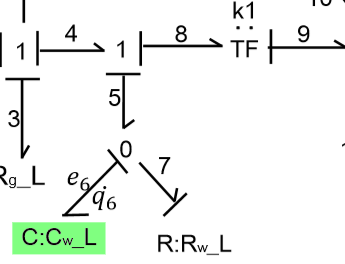
\includegraphics[width=0.4\textwidth]{fig/2_equation2.png}
\end{figure}
%%%%%%%%%%%%%%%%%
对于$\dot{q}_{ 6 }$,开始列写方程,利用键合图的因果关系求出$f_6$:根据功率流方向标注,流变量$f_6$来自0结的输出,是由$f_5$和$f_7$产生的,因此:
\begin{equation}\label{2_f6}
\dot{q}_{6}
=
f_6
=
f_5 - f_7,
\end{equation}
$f_5$直接与状态变量有关;$f_7$同样直接与状态变量有关,故而有下面两式:
\begin{equation}\label{2_f5}
f_5
=
f_4
=
f_2
=
\frac{p_{2}}{J_{w L}},
\end{equation}

\begin{equation}\label{2_f7}
f_7
=
\frac{e_{7}}{R_{w L}}
=
\frac{e_{6}}{R_{w L}}
=
\frac{q_{6}}{C_{wL} R_{w L}},
\end{equation}

由式(\ref{2_f6})-(\ref{2_f7})得到状态方程2:
\begin{equation}\label{2_q6}
\dot{q}_{6}
=
\frac{p_{2}}{J_{w L}}-\frac{q_{6}}{C_{wL} R_{w L}}.
\end{equation}

%%%%%%%%%%%%%%%%%%%%%%%%%%%%%%%%%%%%%%%%%%%%%%%%%%%%%%%%%%%%%%%%
%%%%%%%%%%%%%%%%%%%%%%%%%%%%%%%%%%%%%%%%%%%%%%%%%%%%%%%%%%%%%%%%
%%%%%%%%%%%%%%%%%%%%%%%%%%%%%%%%%%%%%%%%%%%%%%%%%%%%%%%%%%%%%%%%
\item {后轮与整体解耦相关状态变量$\dot{q}_{11}$}
%%%%%%%%%%%%%%%%%
\begin{figure*}[h]
	\centering
	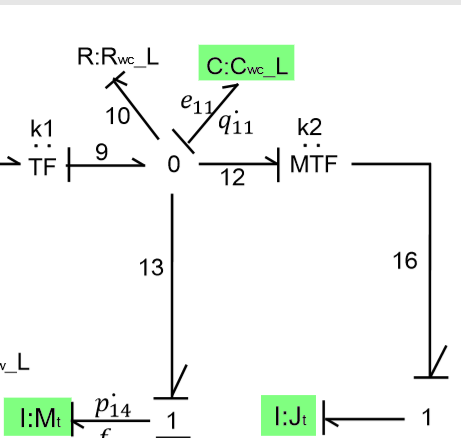
\includegraphics[width=0.4\textwidth]{fig/2_equation3.png}
\end{figure*}
%%%%%%%%%%%%%%%%%
对于$\dot{q} _ { 11 }$,
开始列写方程,通过使用因果关系对$f_11$路径进行跟踪,流变量$f_11$是对$C_{wcL}$的输入,从0结出来的输出,此输出由因果输入$f _ { 9 }$, $ f _ { 10 }$, $  f _ { 12 }$和$f _ { 13 }$产生,因此:
\begin{equation}\label{2_f11}
\dot{q}_{11}
=
f_{11}
=
f_9 - f_{10} - f_{12} - f_{13},
\end{equation}
$f_9$来自TF元件;$f_{10}$来自阻性元件$R _ { wcL }$的输出;$f_{12}$和$f_{13}$同样直接与状态变量有关,故而有下面四式:
\begin{equation}\label{2_f9}
f_{9}
=
f_{8} \cdot k_1
=
f_{4} \cdot k_1
=
f_{2} \cdot k_1
=
\frac{p_{2}}{J_{w L}} k_{1},
\end{equation}

\begin{equation}\label{2_f10}
f_{10}
=
\frac{e_{10}}{R_{wc L}}
=
\frac{e_{11}}{R_{wc L}}
=
\frac{q_{11}}{C_{wc L} R_{wc L}},
\end{equation}

\begin{equation}\label{2_f12}
f_{12}
=
\frac{f_{16}}{k_{2}} 
=
\frac{f_{17}}{k_{2}} 
=
\frac{p_{17}}{J_{t} k_{2}},
\end{equation}

\begin{equation}\label{2_f13}
f_{13}
=
f_{14}
=
\frac{p_{14}}{M_{t}},
\end{equation}

由式\ref{2_f11}-\ref{2_f13}得到状态方程3:
\begin{equation}\label{2_q11}
\dot{q}_{11}
=
\frac{p_{2}}{J_{w L}} k_{1}
-
\frac{q_{11}}{C_{wc L} R_{wc L}}
-
\frac{p_{17}}{J_{t} k_{2}}
-
\frac{p_{14}}{M_{t}}.
\end{equation}

%%%%%%%%%%%%%%%%%%%%%%%%%%%%%%%%%%%%%%%%%%%%%%%%%%%%%%%%%%%%%%%%
%%%%%%%%%%%%%%%%%%%%%%%%%%%%%%%%%%%%%%%%%%%%%%%%%%%%%%%%%%%%%%%%
%%%%%%%%%%%%%%%%%%%%%%%%%%%%%%%%%%%%%%%%%%%%%%%%%%%%%%%%%%%%%%%%
\item {质心处状态分析(质量)状态变量$\dot{ p}_{14} $}
%%%%%%%%%%%%%%%%%
\begin{figure}[H]
	\centering
	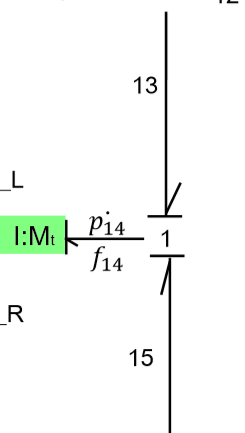
\includegraphics[width=0.25\textwidth]{fig/2_equation4.png}
\end{figure}
%%%%%%%%%%%%%%%%%
对于$\dot{p} _ { 14 }$,开始列写方程,利用键合图的因果关系求出$e_{14}$:根据功率流方向标注,势变量$e_{14}$来自1结的输出,是由$e_{13}$和$e_{15}$产生的,因此:
\begin{equation}\label{2_e14}
\dot{p}_{14}
=
e_{14}
=
e_{13}
+
e_{15},
\end{equation}
$e_{13}$和$e_{15}$均来自容性元件$C _ { wc }$的输出故而有下面两式:
\begin{equation}\label{2_e13}
e_{13}
=
e_{11}
=
\frac{q_{11}}{C_{wc L}},
\end{equation}

\begin{equation}\label{2_e15}
e_{15}
=
e_{20}
=
\frac{q_{20}}{C_{wc R}},
\end{equation}

由式\ref{p13}-\ref{e15}得到状态方程4:
\begin{equation}\label{2_p14}
\dot{p}_{14}
=
\frac{q_{11}}{C_{wc L}}
+
\frac{q_{20}}{C_{wc R}}.
\end{equation}

%%%%%%%%%%%%%%%%%%%%%%%%%%%%%%%%%%%%%%%%%%%%%%%%%%%%%%%%%%%%%%%%
%%%%%%%%%%%%%%%%%%%%%%%%%%%%%%%%%%%%%%%%%%%%%%%%%%%%%%%%%%%%%%%%
%%%%%%%%%%%%%%%%%%%%%%%%%%%%%%%%%%%%%%%%%%%%%%%%%%%%%%%%%%%%%%%%
\item {质心处状态分析(转动惯量)状态变量$\dot{ p}_{17}$}
%%%%%%%%%%%%%%%%%
\begin{figure*}[h]
	\centering
	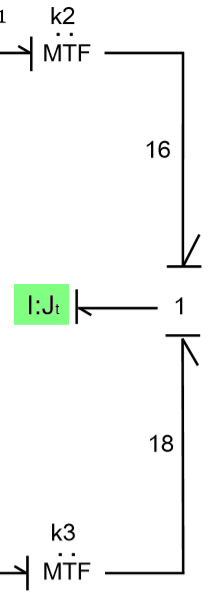
\includegraphics[width=0.25\textwidth]{fig/2_equation5.png}
\end{figure*}
%%%%%%%%%%%%%%%%%
对于$\dot{p} _ { 17 }$,开始列写方程,通过使用因果关系对$p_{17}$路径进行跟踪,从1结出来的输出,此输出由因果输入$e _ { 16 }$和$  e _ { 18 }$产生,因此:
\begin{equation}\label{2_p17}
\dot{p}_{17}
=
e_{17}
=
e_{16}
+
e_{18},
\end{equation}

$e _ { 16 }$和$e_{18}$来自MTF元件的输入,故而有下面两式:
\begin{equation}\label{2_e16}
e_{16}
=
\frac{e_{12}}{k_2}
=
\frac{e_{11}}{k_2}
=
\frac{q_{11}}{C_{w L} k_{3}},
\end{equation}

\begin{equation}\label{2_e18}
e_{18}
=
\frac{e_{19}}{k_3}
=
\frac{e_{20}}{k_3}
=
\frac{q_{20}}{C_{wc R}},
\end{equation}

由式\ref{2_p17}-\ref{2_e18}得到状态方程5:
\begin{equation}
\dot{p}_{17}
=
\frac{q_{11}}{C_{w L} k_{3}}
+
\frac{q_{20}}{k_{2} C_{w R}}.
\end{equation}

%%%%%%%%%%%%%%%%%%%%%%%%%%%%%%%%%%%%%%%%%%%%%%%%%%%%%%%%%%%%%%%%
%%%%%%%%%%%%%%%%%%%%%%%%%%%%%%%%%%%%%%%%%%%%%%%%%%%%%%%%%%%%%%%%
%%%%%%%%%%%%%%%%%%%%%%%%%%%%%%%%%%%%%%%%%%%%%%%%%%%%%%%%%%%%%%%%
\item {根据对称性得到剩余状态方程}
根据对称性,另外三个状态方程可以推出(\ref{2_q20})-(\ref{2_q29}):
\begin{equation}\label{2_q20}
\dot{q}_{20}
=
\frac{p_{29}}{J_{w R}} k_{1}
-
\frac{p_{14}}{M_{t}}
-
\frac{p_{17}}{J_{t} k_{3}}
-
\frac{q_{20}}{R_{wc R} C_{wc R} },
\end{equation}

\begin{equation}\label{2_q25}
\dot{q}_{25}=\frac{p_{29}}{J_{w_{-} R}}-\frac{q_{25}}{R_{w_{-} R} C_{w_{-}} R},
\end{equation}

\begin{equation}\label{2_q29}
\dot{p}_{29}
=
\tau_{R}-\frac{p_{29}}{J_{w R}} R_{g R}
-
\frac{q_{20}}{C_{wc R}} k_{1}
-
\frac{q_{25}}{C_{w R}}.
\end{equation}

\end{enumerate}

\subsection{总体状态空间矩阵}

\subsubsection{状态空间矩阵导出}

下列公式显示了MPW的状态空间表示,其中$ x_1$,$u_1$和$y_1$分别是系统状态,输入和输出:

\begin{equation}\label{2_dot_x1}
\dot{x}_1 =[\mathbf{A}_1] x_1+[\mathbf{B}_1] u_1,
\end{equation}

\begin{equation}\label{2_y1}
y_1 =[\mathbf{C}_1] x_1.
\end{equation}

由上述八个状态空间方程(\ref{2_p2}) ~ (\ref{2_q29}),具体表示成:

\begin{equation}\label{2_matrix1}
\begin{aligned}
\left[ 
\begin{array}
{l}{e_{2}} \\ {f_{6}} \\ {f_{11}} \\ {e_{14}} \\ {e_{17}} \\ {f_{20}} \\ {f_{25}} \\ {e_{25}}
\end{array}
\right] 
=
\left[ 
\begin{array}
{c}{\dot{p}_{2}} \\ {\dot{q}_{6}} \\ {\dot{q}_{11}} \\ {\dot{p}_{14}} \\ {\dot{p}_{17}} \\ {\dot{q}_{20}} \\ {\dot{q}_{25}} \\ {\dot{p}_{29}}
\end{array}
\right]
=
&
\left[ 
\begin{array}{cccccccc}
{- \frac{R_{gL}}{J_{w L}}} & - \frac{1}{C_{wL}} & - \frac{k_1}{C_{w L}} & 0 & 0 & 0 & 0 & 0 \\ 
\frac{1}{J_{w L}} & - \frac{1}{R_{wL} C_{wL}} & 0 & 0 & 0 & 0 & 0 & 0 \\ 
\frac{k_{1}}{J_{W_L}}  & 0 & - \frac{1}{R_{wc L} C_{wc L}} & - \frac{1}{M_{t}} & - \frac{1}{k_{2} J_{t}} & 0 & 0 & 0  \\ 
0 & 0 & \frac{1}{C_{wc L}} & 0 & 0 & \frac{1}{C_{wc R}}  & 0 & 0   \\ 
0 & 0 & \frac{1}{k_{3} C_{wc L}} & 0 & 0 & \frac{1}{k_{2} C_{wc R}}  & 0 & 0  \\ 
0 & 0 & 0 & - \frac{1}{M_{t}} & - \frac{1}{k_{2} J_{t}} & - \frac{1}{R_{wc R} C_{wc R}} & 0 & \frac{k_{1}}{J_{W_R}} \\ 
0 & 0 & 0 & 0 & 0 & 0 & - \frac{1}{R_{w R}  C_{w R}} & \frac{1}{J_{w R}}  \\ 
0 & 0 & 0 & 0 & 0 & - \frac{k_{1}}{C_{wc R}} & - \frac{1}{C_{w R}} &  - \frac{R_{g R}}{J_{wR}} 
\end{array}
\right]
\left[
\begin{array}{c}
{p_{2}} \\ {q_{6}} \\ {q_{11}} \\ {p_{14}} \\ {p_{17}} \\ {q_{20}} \\ {q_{25}} \\ {q_{29}}
\end{array}
\right]
\\
&+
\left[ 
\begin{array}{ll}
{1} & {0} \\ {0} & {0} \\ {0} & {0} \\ {0} & {0} \\ {0} & {0} \\ {0} & {0} \\ {0} & {0} \\ {0} & {1}
\end{array}
\right]
\left[ \begin{array}{l}
{\tau_{L}} \\ {\tau_{R}}
\end{array}\right]
\end{aligned}.
\end{equation}

则输出矩阵则表示为:

\begin{equation}\label{2_matrix2}
\left[
\begin{array}{c}{\omega_{L}} \\ {\omega_{R}} \\ {V_{C G}} \\ {\theta_{C G}}
\end{array}
\right]
=
\left[
\begin{array}{c}{f_{2}} \\ {f_{29}} \\ {f_{14}} \\ {f_{17}}\end{array}
\right]
=
\left[ \begin{array}{cccc}
{\frac{1}{J_{w L}}} & {0} & {0} & {0} \\ {0} & {\frac{1}{J_{w R}}} & {0} & {0} \\ {0} & {0} & {\frac{1}{M_{t}}} & {0} \\ {0} & {0} & {0} & {\frac{1}{J_{t}}}
\end{array}\right] 
\left[ \begin{array}{c}
{p_{2}} \\ {p_{29}} \\ {p_{17}} \\ {p_{17}}
\end{array}\right].
\end{equation}

\subsubsection{特殊变量分析}

特别地,其中的$ k_2 $ 和 $ k_3 $ 属于根据速度变化的动态变量,分别代表转动过程中左右轮相对速度瞬心的曲率半径,需要根据两轮机器人模型导出:

%%%%%%%%%%%%%%%%%
\begin{figure*}[!b]
	\centering
	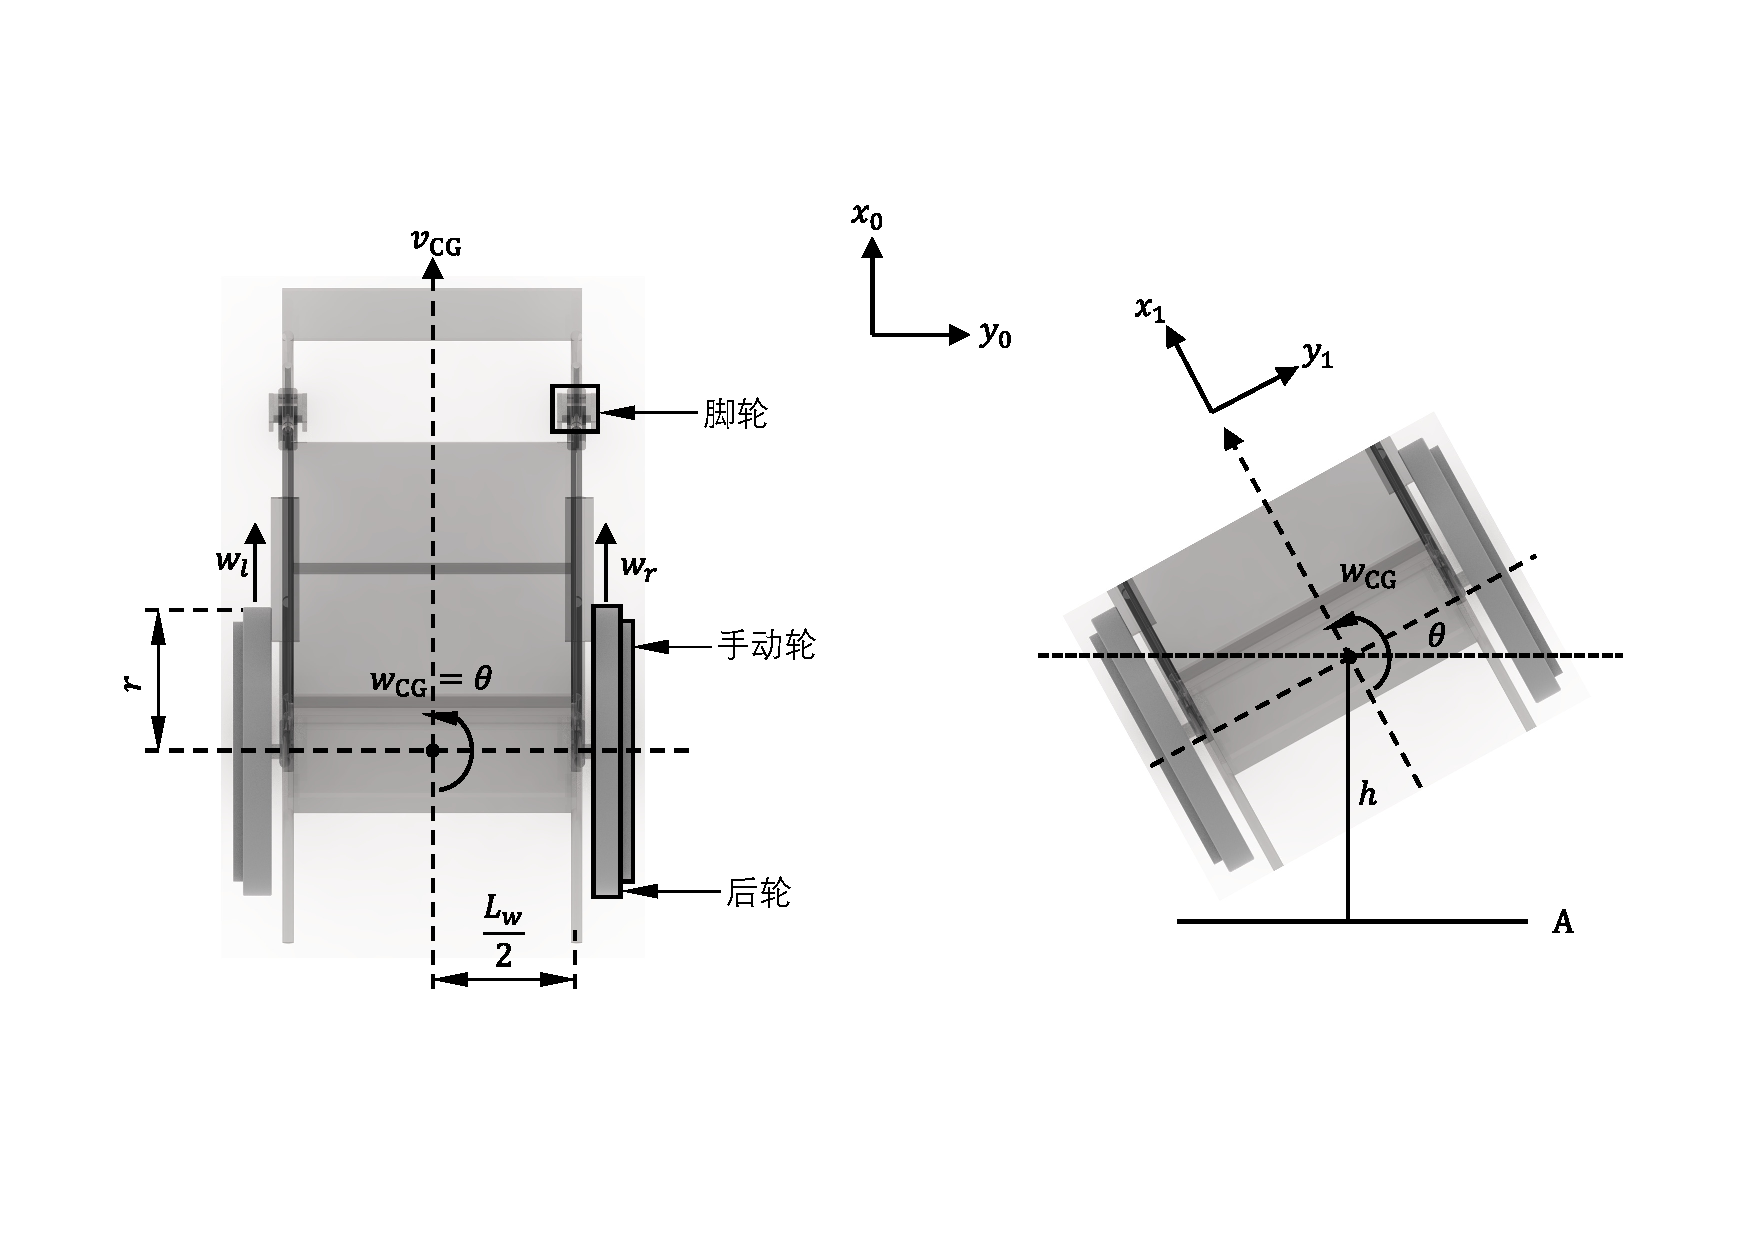
\includegraphics[width=0.95\textwidth]{fig/top_view.pdf}
	\caption{电动轮椅主体俯视示意图。}\label{fig:top_view}
\end{figure*}
%%%%%%%%%%%%%%%%%

在该建模中选取对象的机械主体示意如图 \ref{fig:top_view} 所示。它基本上由两个脚轮和手动后轮组成。在这种建模中已经应用了两轮驱动机器人系统的方法,其中脚轮集中在一起并且假设对系统流施力。 
$ V_{\rm{CG}} $ 和 $ w_{\rm{CG}} $ 代表质心速度和沿质心转速,$ w_l $ 和 $ w_r $ 分别表示左右车轮的角速度,后手动车轮半径和轮椅宽度由 $ r $ 和 $ L_w $ 表示)。
下面的矩阵\ref{equ:basic_eq}显示了系统的运动学数学模型,其中 $ \theta $ 是方位角,$ x $ 和 $ y $ 分别表示系统的几何位置:

%%%%%%%%%%%%%%%%%%%%%%%%%%
\begin{equation}
\label{equ:basic_eq}
\begin{bmatrix} \begin{array}{l}{x} \\ {y} \\ {\theta}\end{array} \end{bmatrix}
=
r
\begin{bmatrix}
\vspace{0.2cm} {\dfrac{\cos \theta}{2}} & {\dfrac{\cos \theta}{2}} \\
\vspace{0.2cm} {\dfrac{2}{L}} & {\dfrac{\sin \theta}{2}} \\
{\dfrac{2}{L_w}} & - {\dfrac{2}{L_w}}
\end{bmatrix}
\begin{bmatrix} \begin{array}{c}{\omega_r} \\ {\omega_l}\end{array} \end{bmatrix}
\ .
\end{equation}
%%%%%%%%%%%%%%%%%%%%%%%%%%

以A作为参考点,左右轮的位移课以得到: 

%%%%%%%%%%%%%%%%%%%%%%%%%%
\begin{equation}
\label{equ:left_s}
S_l = h
-
\frac{L_w}{2} \sin \theta
\ ,
\end{equation}
%%%%%%%%%%%%%%%%%%%%%%%%%%

%%%%%%%%%%%%%%%%%%%%%%%%%%
\begin{equation}
\label{equ:right_s}
S_r = h
+
\frac{L_w}{2} \sin \theta
\ .
\end{equation}
%%%%%%%%%%%%%%%%%%%%%%%%%%

从键合图出发,广义位移变量定义为流变量的时间积分。因此根据上述方程 \ref{equ:left_s} 和 \ref{equ:right_s},可以获得了所需的流变量方程,将可以通过方程 \ref{equ:left_s} 和 \ref{equ:right_s} 用于构建轮椅主体结构的键合图模型。

%%%%%%%%%%%%%%%%%%%%%%%%%%
\begin{equation}
\label{equ:left_v}
v_{l}
=
\dot{S}_{l}
=
\dot{h}
-
\dot{\theta} \frac{L_w}{2} \cos \theta
\ ,
\end{equation}
%%%%%%%%%%%%%%%%%%%%%%%%%%

%%%%%%%%%%%%%%%%%%%%%%%%%%
\begin{equation}
\label{equ:right_v}
v_{r}
=
\dot{S}_{r}
=
\dot{h}
+
\dot{\theta} \frac{L_w}{2} \cos \theta
\ .
\end{equation}
%%%%%%%%%%%%%%%%%%%%%%%%%%

进一步,假设此时$ v_{r} > v_{l} $,则 $ k_3 > k_2 $。根据瞬心的相关几何关系,我们可以得到下列式子:

%%%%%%%%%%%%%%%%%%%%%%%%%%
\begin{equation}\label{equ:k2k3_equs}
\frac{v_L}{k_2} = \frac{v_R}{k_3}.
\end{equation}
%%%%%%%%%%%%%%%%%%%%%%%%%%

其中,由假设与集合关系可得:

%%%%%%%%%%%%%%%%%%%%%%%%%%
\begin{equation}\label{equ:k2k3_Lw}
k_3 = k_2 + L_w.
\end{equation}
%%%%%%%%%%%%%%%%%%%%%%%%%%

结合上述两式可以导出:

%%%%%%%%%%%%%%%%%%%%%%%%%%
\begin{equation}\label{equ:k2_solution}
k_2 = \frac{v_L \times L_w}{v_R - v_L}.
\end{equation}
%%%%%%%%%%%%%%%%%%%%%%%%%%

为了方便编程与建模,上面方程 \ref{equ:k2_solution} 可以写成更一般的形式:

%%%%%%%%%%%%%%%%%%%%%%%%%%
\begin{equation}\label{equ:k2k3}
\begin{aligned}
\min (k_2, k_3) &= \frac{\min (v_L, v_R) \times L_w}{|v_R - v_L|} \\
\max (k_2, k_3) &= \frac{\max (v_L, v_R) \times L_w}{|v_R - v_L|}
\end{aligned}
\end{equation}
%%%%%%%%%%%%%%%%%%%%%%%%%%
